%Write about cloud execution here
\section{Cloud execution}
The size of the problem exceeds the computation resources of a single
virtual machine. We therefore use the HDInsight service on Microsoft
Azure for the full execution.
%% \begin{figure}[!ht]
%%   \centering
%%   
\includegraphics{images/azure}
%%   \caption{HDInsight service on Microsoft Azure}
%%   \label{fig:azure}
%% \end{figure}

We created a cluster with 2 master nodes and 4 computing nodes. Each of
the computing nodes has the configuration of 4 cores CPU, 14GB RAM and
200GB local disk. See Figure~\ref{fig:node}.
\begin{figure}[!ht]
  \centering
  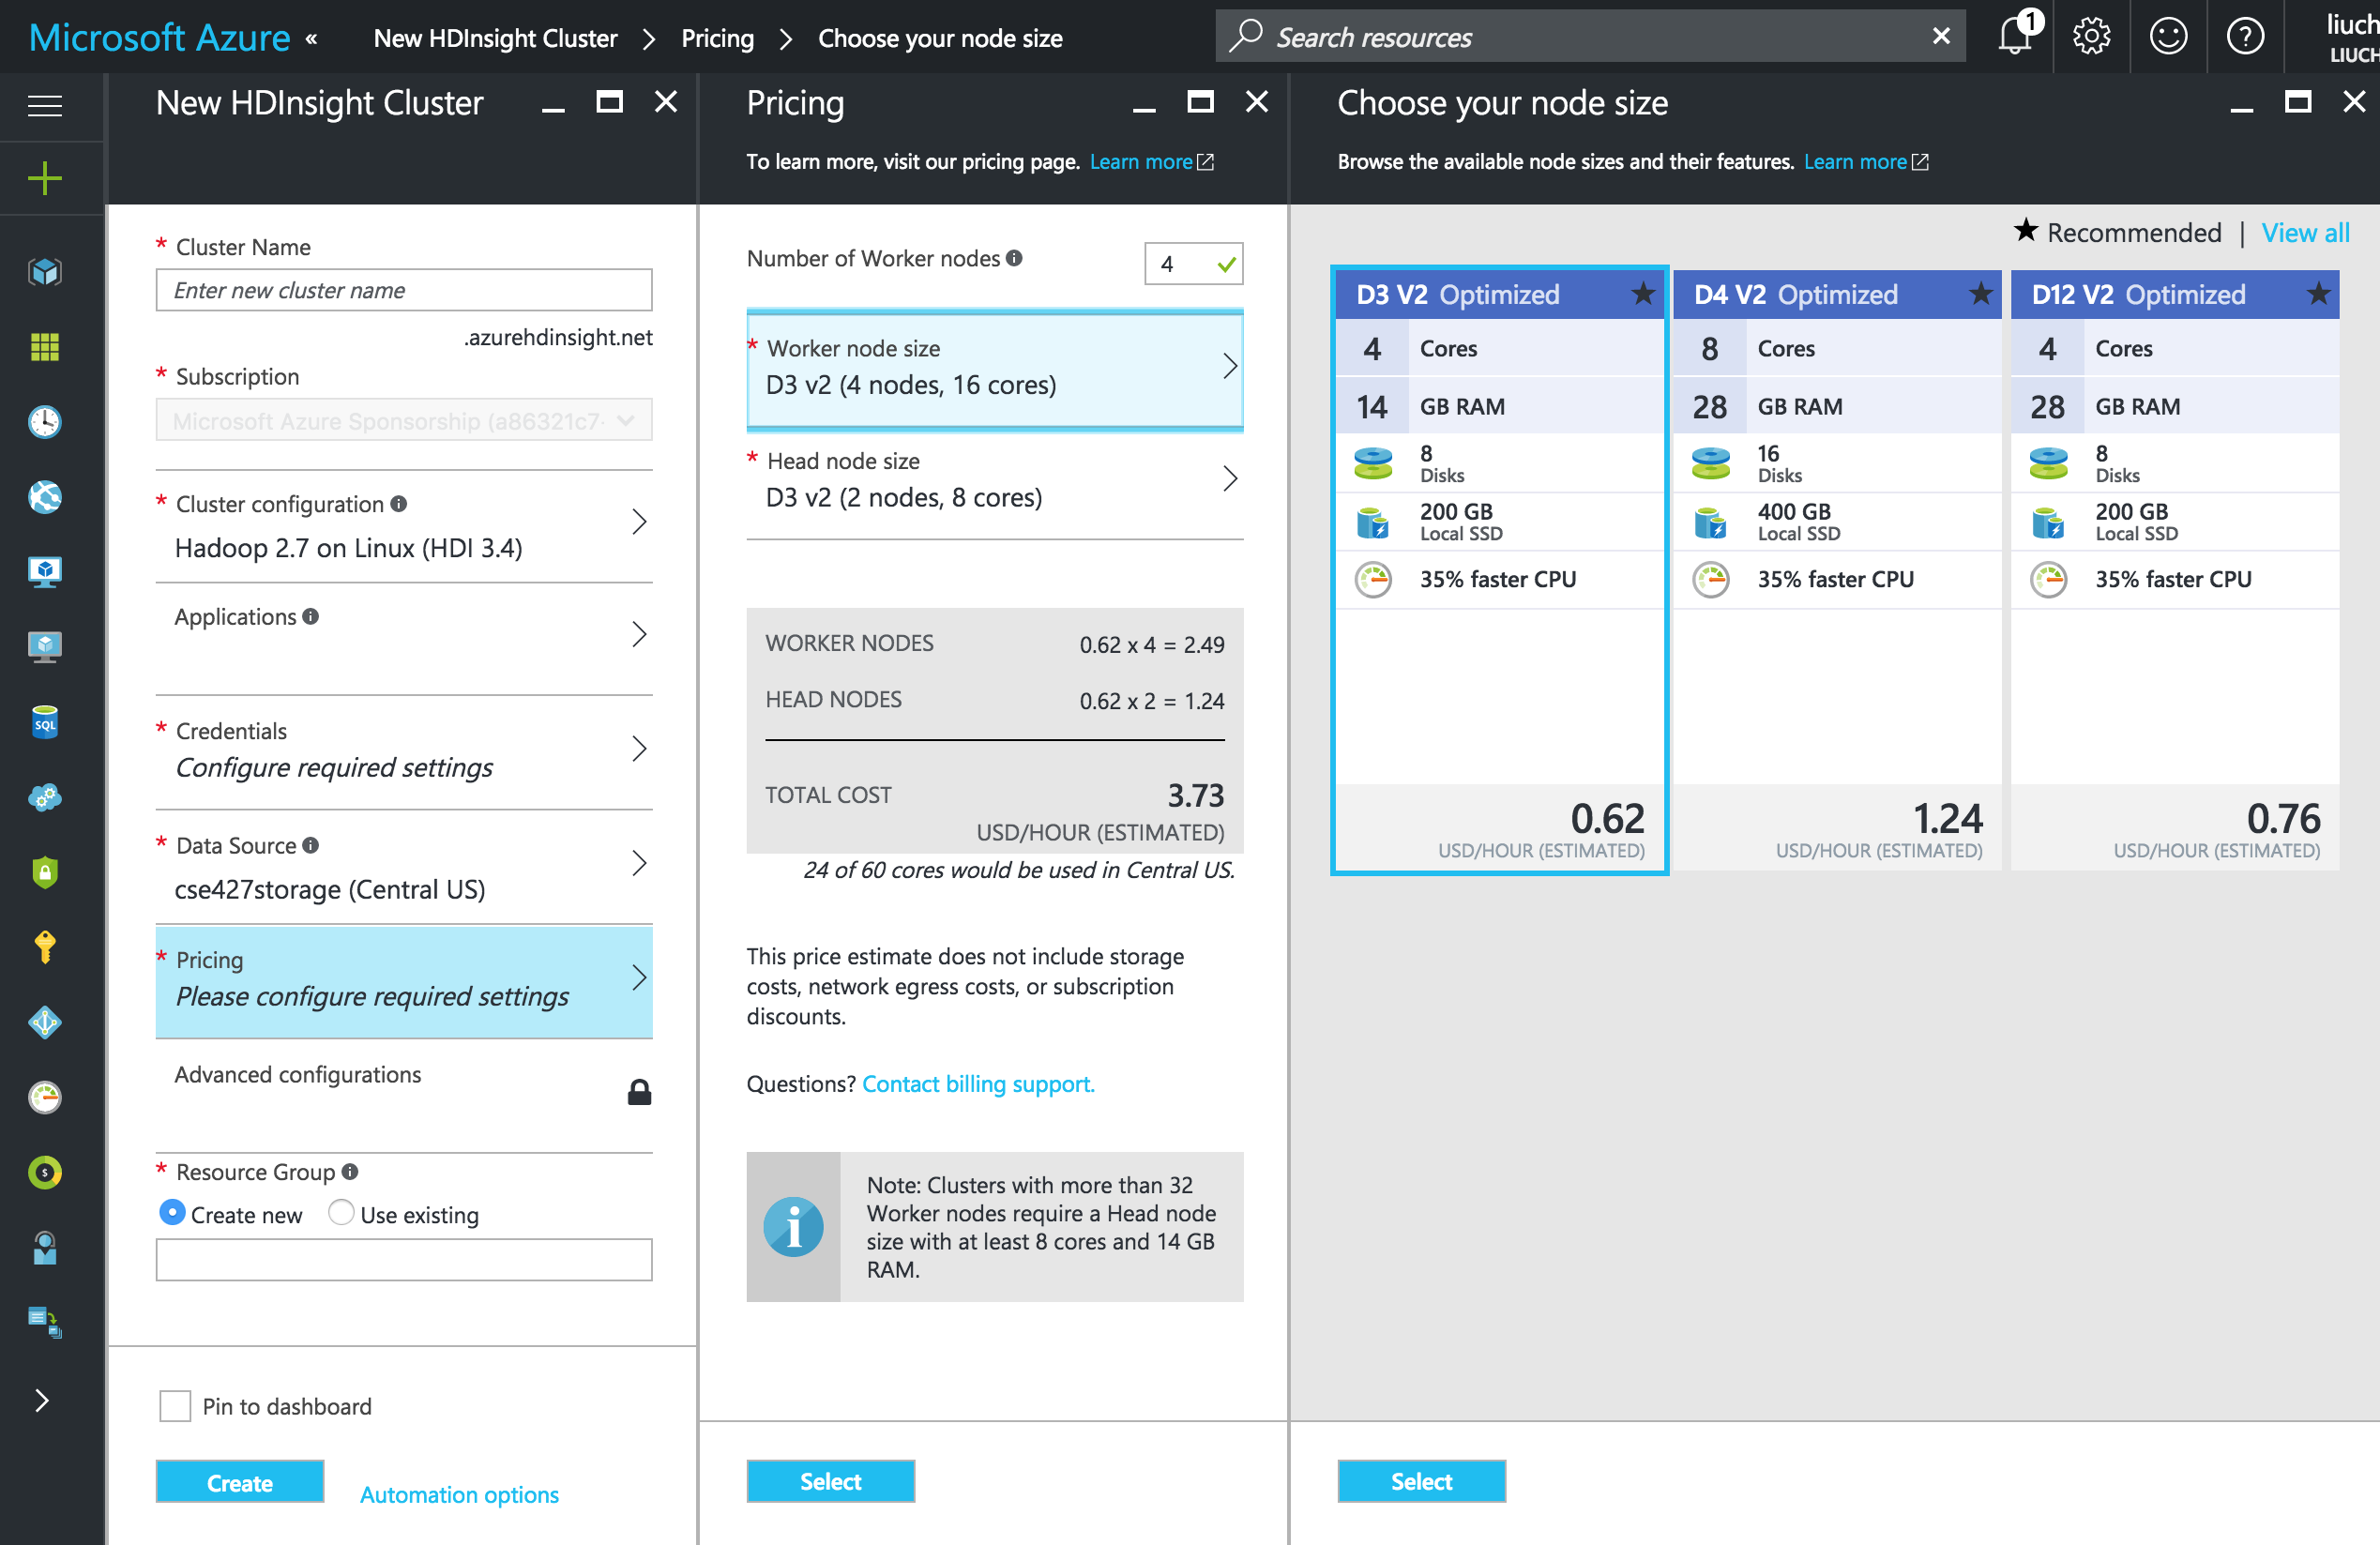
\includegraphics[width=0.95\textwidth]{images/node}
  \caption{Node configuration}
  \label{fig:node}
\end{figure}

The computing time with the cluster is listed in Table~\ref{tab:clustertime}.
\begin{table}[!ht]
  \centering
  \begin{tabular}{|p{2.5cm}|p{4cm}|p{3cm}|p{3cm}|}
    \hline
    Job & Job 1 (item-item pair) & Job 2 (similarity) & Job 3 (top list)\\
    \hline
    CPU Time(s) & 279.55 & 1516.17 & 1100.33\\
    \hline
  \end{tabular}
  \caption{CPU time on the cluster}
  \label{tab:clustertime}
\end{table}
